% template created by: Russell Haering. arr. Joseph Crop
\documentclass[12pt,letterpaper]{article}
\usepackage{anysize}
\usepackage{cite}
\usepackage{amsmath,amssymb,amsfonts}
\usepackage{algorithm}
\usepackage[noend]{algpseudocode}
\usepackage{graphicx}
\usepackage{multirow}
\usepackage{listings}
\usepackage{xcolor}


\marginsize{2cm}{2cm}{1cm}{1cm}

\lstset{ framexleftmargin=9mm, frame=shadowbox,tabsize = 4}

\begin{document}

\begin{titlepage}
    \vspace*{4cm}
    \begin{flushright}
    {\huge
        ECE 375 Lab 4\\[1cm]
    }
    {\large
    	Large Number Arithmetic
    }
    \end{flushright}
    \begin{flushleft}
    Lab session: 015
    
    Time: 12:00-13:50
    \end{flushleft}
    \begin{flushright}
    Author: Astrid Delestine

    Programming partner: Lucas Plastid 

    \vfill
    \rule{5in}{.5mm}\\
    TA Signature
    \end{flushright}

\end{titlepage}

\section{Introduction}
%This is the first Lab in the ECE 375 series and it covers the setup and compilation of an AVR Assembly Program. The student will learn how how to use the sample Basic Bump Bot assembly file and send the binaries to the AVR Microcontroller board. For the second part of the lab the student will be expected to download and compile the included C sample program and from it learn how to configure the I/O ports of the ATmega32U4 Microcontroller. The student will then write their own C program and upload it to the Microcontroller to verify that it runs as expected. The provided programs have been attached in the source code section of this report.
This is the fourth lab in the ECE 375 series and it covers adding and subtracting words as well as multiplying words together. In this sense words designate 16 bit numbers. It is important to note that this assembely was written for the m128 chipset and not the regular atmetga32u4 chipset. This is due to the fact that we can operate a simulation tool when using the m128 chipset that is not avalabe when we use our regular chipset.

\section{Design}
To design the program for this lab, Lucas and I brainstormed exactly what needed to happen and how we wanted it to go. We needed to determine what the buttons were going to do, and so with the main guide's and the presentation slides, we planned to have four different buttons clear the display, set the display to static text, scroll through the display in a marquee fashion and halt the marquee function when needed. Below one can see a block diagram of what our original plan was.

\begin{figure}[h]
	%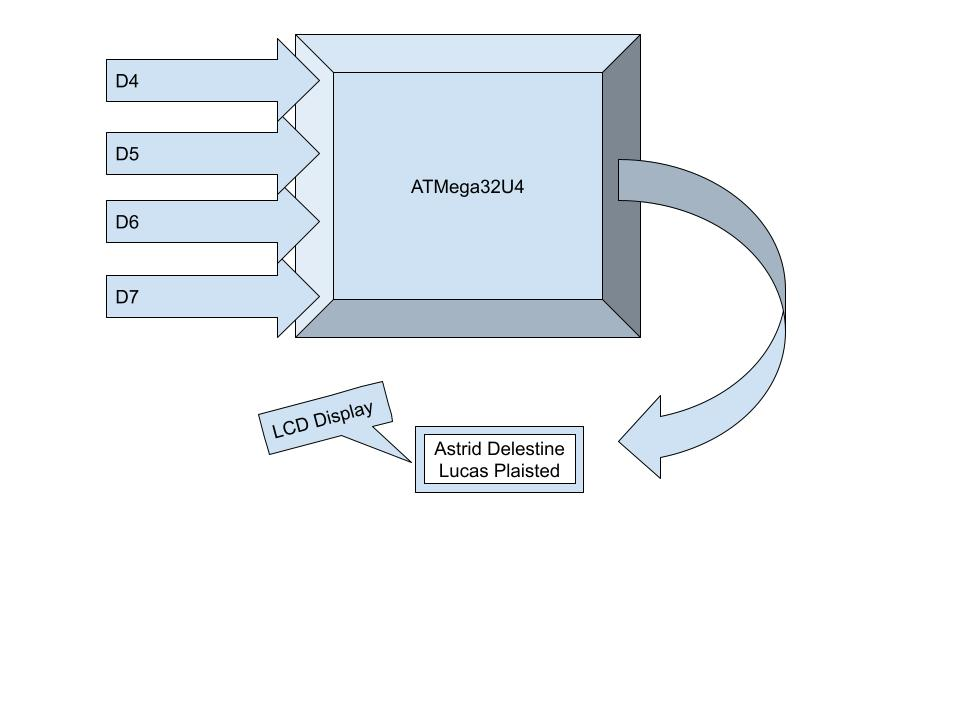
\includegraphics[width=12cm, height=10cm]{BlockDiagramLab3.jpg}
	\centering
\end{figure}
	
\section{Assembly Overview}
As for the Assembly program an overview can be seen below

\subsection{Internal Register Definitions and Constants}
The multipurpose register was setup as r16. a wait counter register was setup at r17. For the timer function an inner counter and outer counter register were setup as r18 and r19 respectively. Several different values of importance were also named such as the LCD memory locations for the first line, the second line, and the end of the second line. 

\subsection{Initialization Routine}
Firstly the stack pointer is initialized, next the LCD display is initialized via an rcall. Finally the port D is initialized to have all inputs. 

\subsection{Main Routine}
The main routine is quite simple, First a function is called BTN2MPR, then using the output of this function, expected to be saved to mpr, we can compare particular bits to see if buttons have been pressed. If a button, say button d5 is pressed, then an rcall is made to DISPNAMES. This will continue to loop until the end of time. 


\subsection{Subroutines}
	\subsection{MARQUEE}
	The marquee function will shift letters from their current locations to the right and if they go off the screen they will loop around. This will happen at a stock rate of 1 movement per quarter second. This can be adjusted. Marquee will continue until button 6 is pressed. First the function loads the display with all the characters then it goes into its main loop, rotating the characters back and forth, and making sure to write to the LCD in between each moment. Some added functionality of this subroutine is that we can speed up or slow down the marquee if necessary. Once button 6 has been pressed the loop will end and the function returns to the main or wherever called it. 
	
	\subsection{ROTCHAR}
	ROTCHAR rotates all charters right through the memory where the LCD pulls from. It does not write to the display it only edits the memory locations. It preforms this action by pushing the variables it is going to use to the stack for safe keeping, then it loads the LCD Ends into the Y pointer. It then pulls the last character and saves it into mpr and pushes it to the stack. Mpr is then loaded with the pre-decremented location of Y, causing the letter before last to be saved into mpr. it is then moved up by 1 in memory, and this will continue until the first character is moved, then the loop breaks and the first character is set to the character previously pushed to the stack. Finally all variables are popped back to their previous locations and the program counter returns to where it was before.  


	\subsubsection{BTN2MPR}
	Places the 4 button inputs into the higher 4 bits of mpr. These buttons are active low. To confirm that it is only the 4 top most bits being saved into mpr an and filter is applied before returning to the main function. 
	
	\subsubsection{DISPNAMES}
	This subroutine is quite simple, it first pushes all the variables it is going to use onto the stack. Then it loads the string locations into the Z pointer, it also loads the LCD locations into the Y pointer. Then using mpr it copies data from the Z pointer to the LCD location 1 letter at a time, until both the top and the bottom buffers have been filled. then it calls the lcd write function, and finally pops all the saved variables off the stack before returning back to the previous function. 
	
	\subsubsection{Wait}
	The Wait subroutine controls the wait intervals while another function is preforming an action. Due to each clock cycle taking a measurable amount of time, we can calculate how many times we need to loop for. This function used the olcnt and ilcnt to have two nested loops, running the dec command until they equal zero, thus waiting the requested amount of time. \textbf{The original program was changed by modifying the Wtime constant value by shifting the bit back by 1 space inside of the HitRight subroutine and the HitLeft subroutine. This effectively doubles the wait time. See Lines 167, 201}


\section{Testing}
Tested each button
\begin{table}[h]
	\centering
	\begin{tabular}{|l|l|l|ll}
		\cline{1-3}
		Case & Expected & Actual meet expected &  &  \\ \cline{1-3}
	D4 Pressed	&Clears the Display&	\checkmark  &  \\ \cline{1-3}
	D5 Pressed	&Shows 2 lines of text, Each name&	\checkmark	&  \\ \cline{1-3}
	D6 Held after D7 is Pressed	&Cancels Marquee&	\checkmark  &  \\ \cline{1-3}
	D7 Pressed	&Begins Marquee&	\checkmark	&  \\ \cline{1-3}
	
%		&          &                      &  &  \\ \cline{1-3}
	\end{tabular}
\caption{Assembly Testing Cases}
\end{table}

\section{Study Questions}
\begin{enumerate}
    \item
    Although we dealt with unsigned numbers in this lab, the ATmega32 micro-controller also has some features which are important for performing signed arithmetic. What does the V flag in the status register indicate? Give an example (in binary) of two 8-bit values that will cause the V flag to be set when they are added together.
    
    \item 
    In the skeleton file for this lab, the .BYTE directive was used to allocate some data memory locations for MUL16’s input operands and result. What are some benefits of using this directive to organize your data memory, rather than just declaring some address constants using the .EQU directive?
    \item 
    In computing, there are traditionally two ways for a microprocessor to listen to other devices and communicate: polling and interrupts. Give a concise overview/description of each method, and give a few examples of situations
    where you would want to choose one method over the other.    
    \item
	Describe the function of each bit in the following ATmega32U4 I/O registers: EICRA, EICRB, and EIMSK. Do not just give a brief summary of these registers; give specific details for each bit of each register, such as its possible values and what function or setting results from each of those values. Also, do not just directly paste your answer from the datasheet, but instead try	to describe these details in your own words.
    
	\item 
	The ATmega32U4 microcontroller uses interrupt vectors to execute particular instructions when an interrupt occurs. What is an interrupt vector? List the interrupt vector (address) for each of the following ATmega32U4 interrupts: Timer/Counter0 Overflow, External Interrupt 6, and Analog Comparator.
	
	
	
	
	\item 
	Microcontrollers often provide several different ways of configuring interrupt triggering, such as level detection and edge detection. Suppose the signal shown in Figure 1 was connected to a microcontroller pin that was configured
	as an input and had the ability to trigger an interrupt based on certain signal conditions. List the cycles (or range of cycles) for which an external interrupt would be triggered if that pin’s sense control was configured for: (a) rising
	edge detection, (b) falling edge detection, (c) low level detection, and (d) high level detection. Note: There should be no overlap in your answers, i.e., only one type of interrupt condition can be detected during a given cycle.
	
	

\end{enumerate}

\section{Difficulties}
This lab was not too difficult, however determining exactly how the marquee needed to work was definitely a challenge. After sorting out the bugs, it was extremely exciting to see text show up on the display.  

\section{Conclusion}
This lab really helped teach just how peripherals can work, and how the ATMEGA32U4 handles certain peripherals. Several parts were challenging however these stimulating moments allowed the student to learn and understand what they needed to do at the same time. 

\section{Source Code}%
\lstinputlisting
[
caption=Assembely Bump Bot Script,
language={[x86masm]Assembler},
numbers =left,
rulesepcolor=\color{blue}
]{../Lab4Assm/Lab4Assm/Astrid_Delestine_and_Lucas_Plaisted_Lab4_sourcecode.asm}





\end{document}